
%%%%%%%%%%%%%%%%%%%%%%%%%%%%%%%%%%%%%%%%%%%%%%%%%%%%%%%%%%
%%
%% MARK: Title
%%
%%%%%%%%%%%%%%%%%%%%%%%%%%%%%%%%%%%%%%%%%%%%%%%%%%%%%%%%%%

\chapter*{\S B25. Klein Stratification of Diffeological Spaces}
\setcounter{footnote}{0}

%%%%%%%%%%%%%%%%%%%%%%%%%%%%%%%%%%%%%%%%%%%%%%%%%%%%%%%%%%
%%
%% MARK: Abstract
%%
%%%%%%%%%%%%%%%%%%%%%%%%%%%%%%%%%%%%%%%%%%%%%%%%%%%%%%%%%%

\begin{abstract}
  In this note we see that every diffeological space is naturally stratified by the action of its diffeomorphisms.
\end{abstract}

%%%%%%%%%%%%%%%%%%%%%%%%%%%%%%%%%%%%%%%%%%%%%%%%%%%%%%%%%%
%%
%% MARK: Klein Stratifications
%%
%%%%%%%%%%%%%%%%%%%%%%%%%%%%%%%%%%%%%%%%%%%%%%%%%%%%%%%%%%
\section{Klein stratifications}

As we already know,
diffeology is a flexible category,
stable by any set-theoretic operation.
In particular diffeology gives a simple and natural access to singularities,
as many examples already have shown \cite{DI83, IKZ10, PIZ15},
even when the space is topologically trivial the diffeology can be relevant,
which is the case for irrational tori for example \cite{DI83}.%
\footnote{This remarkable property has important consequences since it allows theorems that could not exist otherwise.
For example,
one proved that every symplectic manifold is an orbit of the linear coadjoint action of a central extension of the group of hamiltonian diffeomorphisms by the torus of periods of the symplectic form,
which is in general not a manifold but trivial as topological space \cite{DIZ22}.}

In the case of irrational torus,
the singularity lies in the global nature of the space,
and comes from the discrepancy between its trivial topology and its non-trivial diffeology.
On the other hand,
from a local point of view,
the diffeology of a space encodes in a strong way,
the internal singularities of the space.
They are revealed by the action of the diffeomorphisms.
For example,
in a square a diffeomorphism can exchange only vertices and edges and fixes the interior.
Without claiming that this Kleinian perspective exhausts the nature of geometry,
it provides a powerful way to reveal the internal singularities of a diffeological space.

This remark gave rise to the first definition of Klein strata of a diffeological space,
as the orbits of the group of diffeomorphisms.
We recall this definition from \cite[\textsection\,1.42]{PIZ13}.

\begin{Article}{Definition 1.}{}
  Let $X$ be a diffeological space,
  the \emph{Klein strata} of $X$ are defined as the orbits of $\Diff(X)$,
  its group of diffeomorphisms.
\end{Article}

An important remark that did not appear in the book in the section 1.42 devoted to Klein's strata is the following:

\begin{Article}{Proposition 1.}{}
  The Klein strata of a diffeological space $X$,
  defined as the orbits of its group of diffeomorphisms,
  form a stratification in the sense that the closure of a Klein stratum,
  for the D-topology,
  is a union of Klein strata.
  In other words,
  if $\cO$ is an orbit of $\Diff(X)$,
  then there exists a subset $\Sigma \subset X$ such that
  $$
    \overline\cO = \bigcup_{x \in \Sigma} \cO_x,
    $$
  where $\cO_x$ denotes the orbit of $x$ and $\overline\cO$ the closure of $\cO$.
\end{Article}

The D-topology has been defined originally in \cite{Igl85} and also in \cite[\textsection\,2.8]{PIZ13}.
This is the finest topology for which the plots are continuous.
A subset $\cO \subset X$ is open for the D-topology,
or is a \emph{D-open},
if $P^{-1}(\cO)$ is open in $\Domain(P)$ for all plots $P$ in $X$.
%
The previous proposition can be stated as follows:

\begin{Article}{Proposition 1 bis.}{}
  Let $\cO_x$ and $\cO_y$ be two orbits by the group $\Diff(X)$.
  If $x \in \overline{\cO_y}$ and $x' \in \cO_x$,
  then $x' \in \overline{\cO_y}$.
\end{Article}

\begin{proof}
  The proof is straightforward:
  since diffeomorphisms are homeomorphisms \cite[\textsection\,2.9]{PIZ13},
  the closure relation is preserved by diffeomorphisms.
  The following is just given to make this statement obvious.
  
  \begin{figure}[t]
    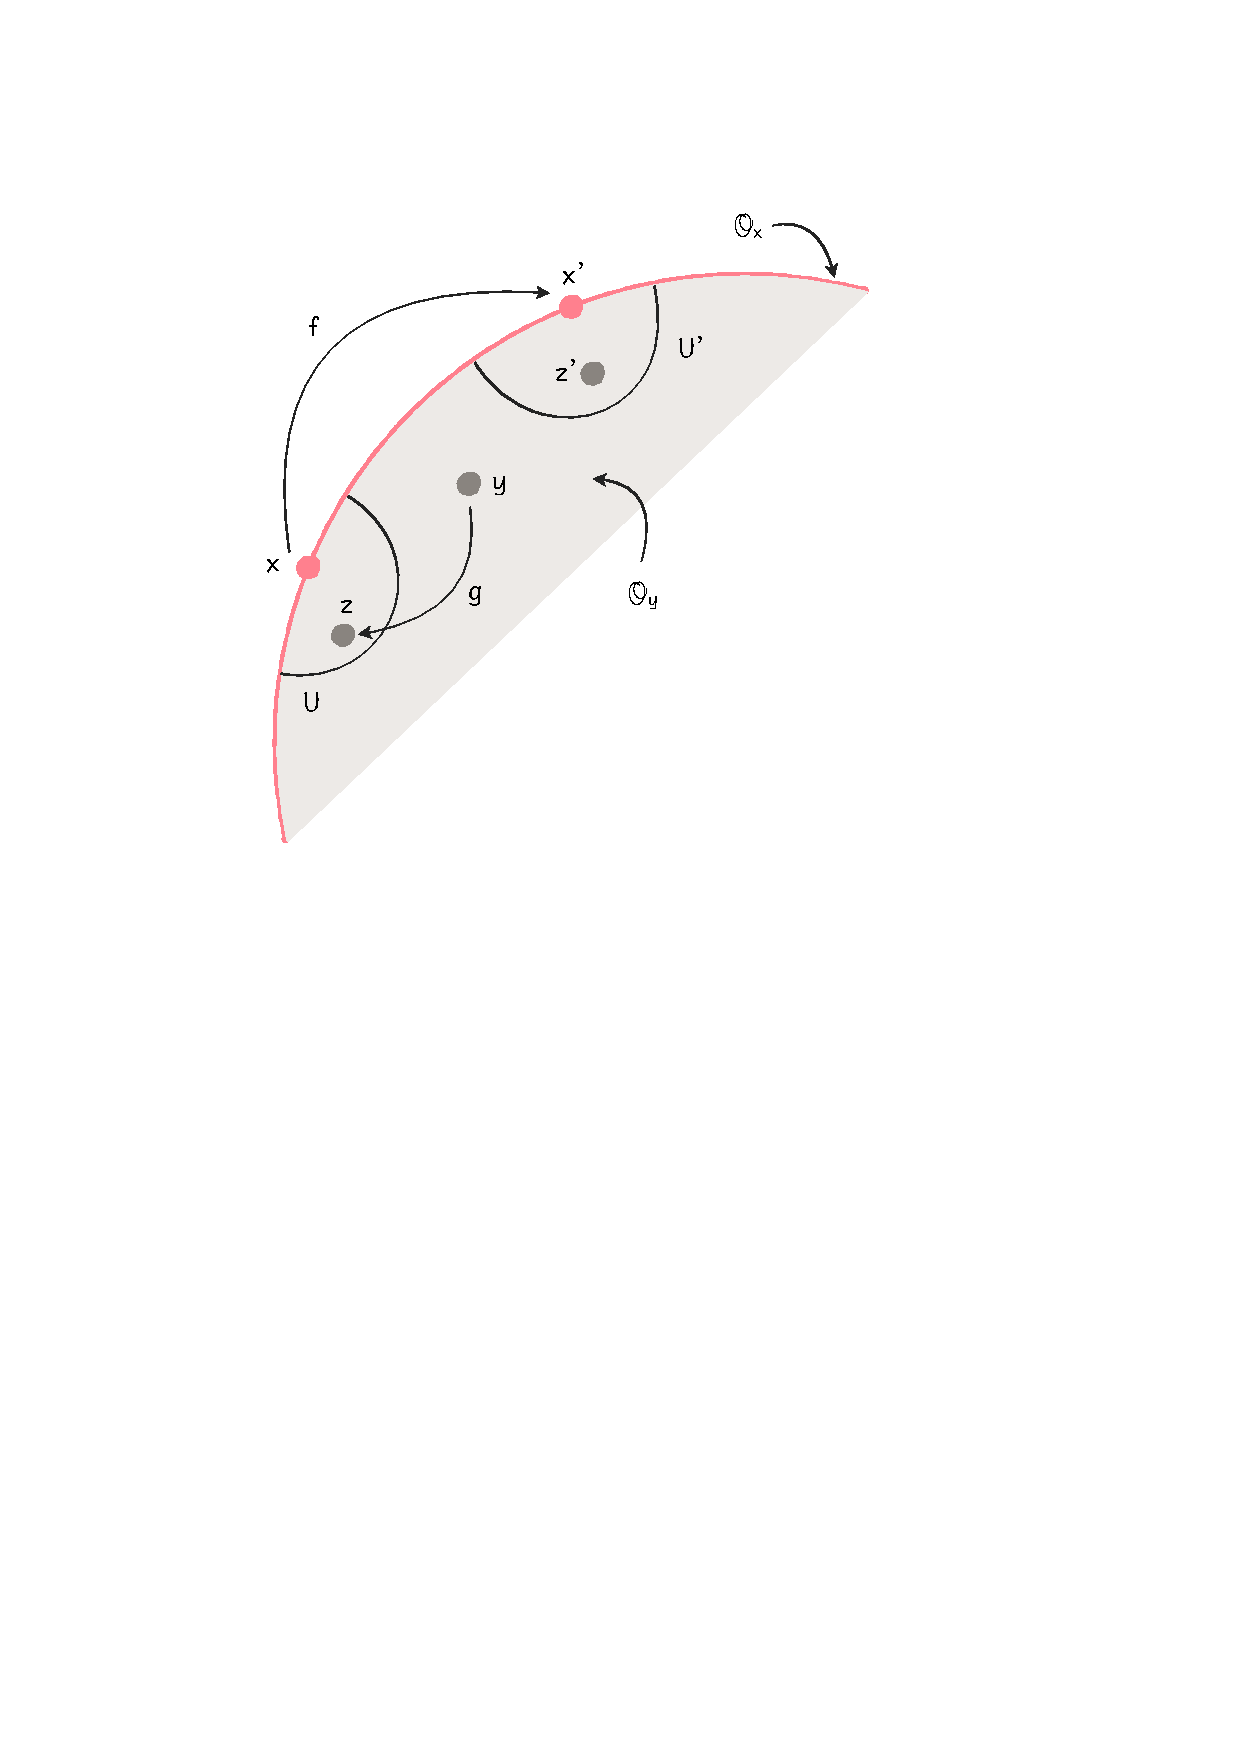
\includegraphics[width=.5\textwidth]{Figures/Frontier-condition.pdf}
    \vspace{-.25\baselineskip}
    \caption{The frontier condition.}
    \label{Frontier-condition.pdf}
\end{figure}
  
  Let $U'$ be a D-open neighborood of $x'$.
  Since $x' = f(x)$,
  with $f \in \Diff(X)$,
  $U = f^{-1}(U')$ is a D-open neighborhood of $x$.
  Then,
  there exists $z = g(y) \in \cO_y \cap U$.
  Thus
  $z' = f(z)$ belong to $U' = f(U)$ and $z' \in \cO_y$,
  since $z \in \cO_y$ and $z' = f(z)$.
  Therefore $U' \cap \cO_y \neq \varnothing$.
\end{proof}

Consider the example of the square $\Sq$ described in Figure \ref{The diffeomorphisms of the square}.
The group $\Diff(\Sq)$ has \uline{three orbits}:

\begin{enumerate}
  \item[1.] the 4-corners-orbit;
  \item[2.] the 4-edges-orbit;
  \item[3.] the interior-orbit.
\end{enumerate}

The first remark we can do here is that the corners orbits,
and the edges orbit,
are not connected but their elements can be treated separately.
Indeed,
it is sufficient to redefine the Klein strata:

\begin{Article}{Definition 1 bis.}{}
  Let $X$ be a diffeological space,
  the connected \emph{Klein strata} of $X$ are defined as the orbits of $\Diff(X)^0$,
  the identity component of the group of diffeomorphisms of $X$.
\end{Article}

Connected Klein strata are indeed connected.
They are the images of a connected diffeological group by a smooth \emph{orbit applications} $\hat x : f \mapsto f(x)$.

In the case of the square there are now \uline{nine strata}:

\begin{enumerate}
  \item[1.] Four corners: NE, SE, SW, NW;
  \item[2.] Four edges: NE---SE, SE---SW, SW---NW, NW---NE;
  \item[3.] One interior.
\end{enumerate}

As a remark,
the partition of $X$ into connected Klein strata is still a stratification in the sense that it satisfies the frontier condition,
for the same reason of proposition 1.

\begin{Article}{Proposition 2.}{}
  The connected Klein strata of a diffeological space $X$,
  defined as the orbits of the identity component of its group of diffeomorphisms,
  form a stratification in the sense that the closure of a Klein stratum is a union of Klein strata.
\end{Article}

These few previous considerations suggest a broadening of the definition of these stratifications:

\begin{Article}{Definition 2.}{}
  Let $X$ be a diffeological space,
  Let $G$ be any diffeological group acting on $X$ by a smooth homomorphism $g \mapsto g_X$.
  The orbits of the action of $G$ on $X$ form a \emph{geometric stratification} that satisfies the frontier condition.
\end{Article}

\begin{proof}
  Identical to Proposition 1.
\end{proof}

Now,
the notion of stratification goes hand in hand with that of singularity.
The idea of singularity is by definition local.
We consider then the local geometry of a diffeological space:
it is defined at each point by the germ of the diffeology there.%
\footnote{That can be defined precisely.}
The local geometry at each point is preserved by the action of local diffeomorphisms,
which is no more a group but a so-called pseudo-group,
we denote it by $\Diff_\loc(X)$.
Local diffeomorphisms can exchange only points with the same local geometry.
That leads to the following definition:

\begin{Article}{Definition 3.}{}
  Let $X$ be a diffeological space.
  We call \emph{local Klein strata} the orbits of its local diffeomorphisms.
\end{Article}

In other words,
Klein strata gather the points that share the same local geometry.

\begin{Article}{Proposition 3.}{}
  The local Klein strata of a diffeological space $X$,
  defined as the orbits of the local diffeomorphisms,
  form a stratification in the sense that the closure of a Klein stratum is a union of Klein strata.
\end{Article}

\begin{proof}
  Identical to Proposition 1 since local diffeomorphisms are defined on D-open subsets.
\end{proof}

%%%%%%%%%%%%%%%%%%%%%%%%%%%%%%%%%%%%%%%%%%%%%%%%%%%%%%%%%%
%%
%% MARK: Klein Stratifications and Singularities
%%
%%%%%%%%%%%%%%%%%%%%%%%%%%%%%%%%%%%%%%%%%%%%%%%%%%%%%%%%%%
\section{Singularities}

Local Klein strata are associated with the idea of \emph{singularity}.
In some sense they capture the singular points of the diffeological space.
However,
the singularity here is a relative concept,
a point is not singular by itself but relatively to others.
This means,
in the example of the square,
that the corners are singular to the interior points,
as are the edges,
but they are not equivalent to each other.

The precise definition of singularity dwells in the definition of preorder associated with every geometric stratification,
and eventually with the local Klein strata.

\begin{Article}{Proposition 4.}{}
  The binary relation defined on the space of local Klein strata by
  $$
    \cO \preceq \cO' \quad \text{iff} \quad \cO \subset \overline{\cO'}
    $$
  is a natural \emph{preorder},
  that is,
  reflexive and transitive.
  One can say that $\cO$ is \emph{singular} with respect to $\cO'$ if $\cO \preceq \cO'$.
  The set of strata is called a PrOSet.
\end{Article}

It appears that the space of local Klein strata,
equipped with the quotient diffeology,
is an Alexandrov topological space for this preorder.
This preorder is a partial order (reflexive, transitive and antisymetric) if and only if the D-topology of the space of strata is $T_0$-separated.
It has been shown that this is equivalent for the strata to be locally closed when the projection map is open,
see \cite{SY19} for example.
In this case we say that the space of strata is a POSet.

\begin{Article}{Example of a PrOSet.}{}
  The \emph{solenoid} action of $\RR$ on the 2-torus:
  $$
    \underline{t}(z,z') = \big(z e^{2i\pi t}, z' e^{2i\pi \alpha t}\big)
    $$
  gives a POset if $\alpha \in \QQ$ and only a PrOSet otherwise,
  if $\alpha \in \RR - \QQ$.
  In this case, every stratum is in the closure of every other one,
  that is,
  the whole torus $\Torus^2$.
\end{Article}

\begin{Article}{Example of a POSet}{}
  The space of strata of the square is a POset.
  There are four minimal strata of the following type:
  
  \begin{center}
    \begin{tikzcd}
      {}          & \text{NW---NE} \arrow[dl] & {} \\
      \text{NW}   & {}                        & \text{Int} \arrow[ul] \arrow[dl] \\
      {}          & \text{NW---SW} \arrow[ul] & {}
    \end{tikzcd}
  \end{center}
  where the arrow is for $\preceq$.
  The vertices NW, NE, SE, SW are the minimal points.
\end{Article}

%%###########
\begin{figure}[htb]
  \centerline{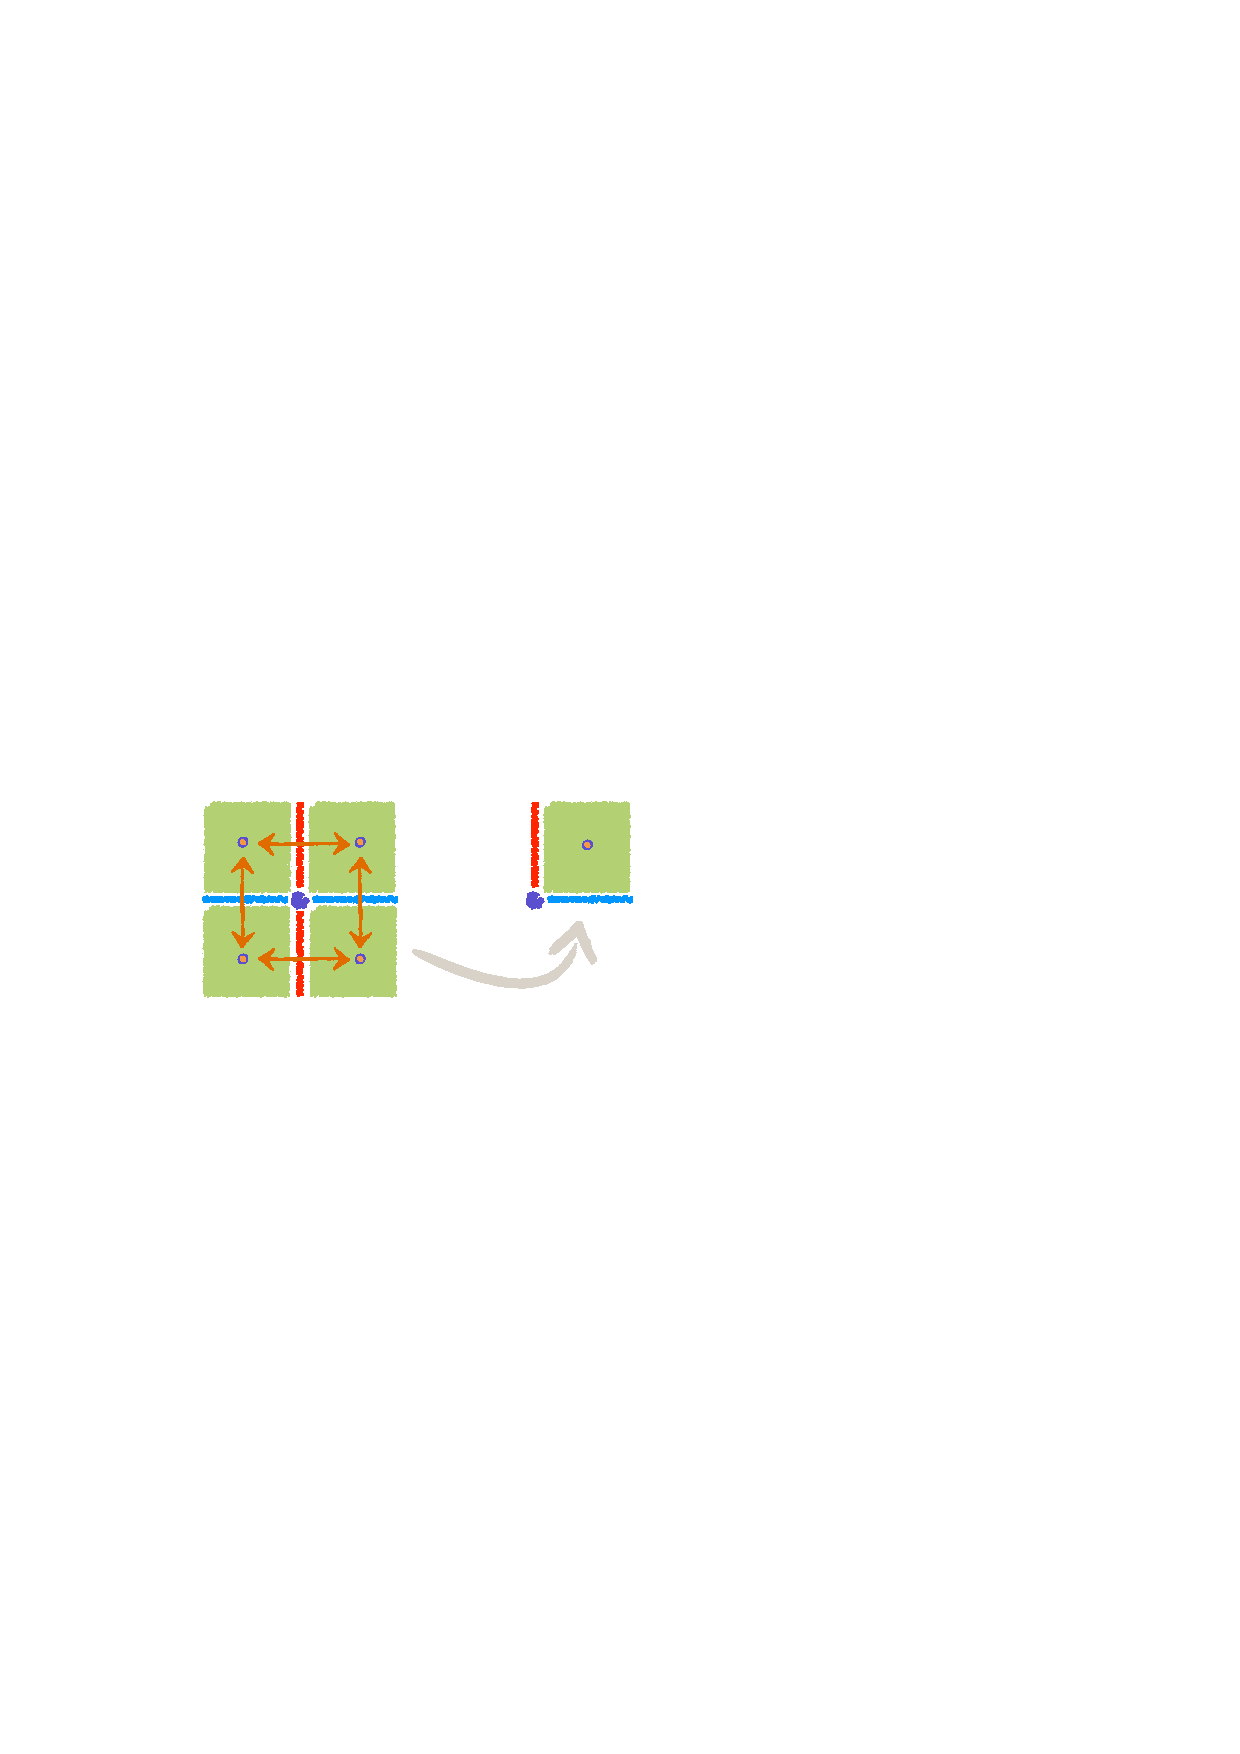
\includegraphics[width=.75\textwidth]{Figures/Corner-orbifold.pdf}}
  \caption{The corner orbifold $\RR^2/\{\pm1\}^2$.}
  \label{The corner orbifold}
\end{figure}
%%###########

\Note An interesting application of this subject would be the analysis of the Klein stratification of the space of orbits of a manifold $M$
by the action of a compact group $G$.
In particular,
to compare the stratification of $M$ by type of stabilizer and the Klein stratification of $M/G$.
We have studied, with Serap Gürer,
the Klein stratification of an orbifold \cite{GIZ22},
see Figure \ref{The corner orbifold} for example,
and we have proved that it coincides with the orbit type stratification.

%\vfill\n
%\centerline{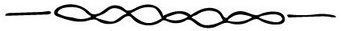
\includegraphics[width=.5\textwidth]{Figures/separator-2.jpg}}\n
%\vfill\n
